% -*- encoding: UTF8 -*-
%%*****************************************************************************
%%									                    	Theoretical Basics								 
%%*****************************************************************************

\chapter{Theory}
\label{Ch:Theory}	

This work combines several principles of optics and mechanics to create an imaging device. Therefore, a review of some relevant theoretical fundamentals will ease the understanding of the design and functionality of the presented device.

Starting with the optical design, the probe uses the concept of Fourier Domain Optical Coherence Tomography (SD-OCT) to extract the depth information of the sample and the mechanism of Laser Scanning Microscopy (LSM) to acquire its lateral information. A LSM needs a scanning mechanism to displace laterally the focus position of an optical imaging device. In this work, this displacement is achieved by a tube shaped actuator which uses the piezoelectric effect to drive a thin resonant beam into resonance.

\section{Optics}
Optical coherence tomography (OCT) is a confocal, interferometric measurement method which allows the retrieval of depth information of a sample from its backscattered light. Due to its non-invasive nature, it is used in an expanding variety of medical imaging methods. Although there are extensive introductions to OCT, i.e. by Drexler and Fujimoto {\cite{Drexler2008}, this section briefly describes the underlying physical mechanism of OCT and confocal imaging.

\subsection{Fourier domain OCT}
The core functionality of OCT is implemented using a Michelson interferometer, as depicted in \autoref{fig:OCTsch}.

\begin{figure}[h!]\centering \includegraphics{figures/20_Theory/Optical/SSOCT-Schema.pdf}
      \caption{Schematic of a SS-OCT measurement system based on a Michelson interferometer, where the sample is modeled as a discrete number of reflectors at different depths and reflectivities. Modified with permision from \cite{Kretschmer}}
      \label{fig:OCTsch}
\end{figure}

In swept-source OCT (SS-OCT), a type of Fourier Domain OCT, the light source used in the interferometer originates from a narrowband laser with the ability to tune its wavenumber $k = \frac{2 \pi}{\lambda}$ over a wide range. To gain intuition on how SS-OCT can extract depth information,  consider a single reflector placed in the measurement arm at a distance $z_{\mathrm{M1}}$. The intensity measured by the detector due to this mirror is described by the two beam interference equation
\begin{equation}
I_{\rm{D}}(k)=I_{\rm{M1}}+I_{\rm{R}}+\sqrt{I_{\rm{M1}}\,I_{\rm{R}}}\,cos\left(2\,k\,\left(z_{\rm{M1}}-z_{\rm{R}}\right)\right).
\end{equation}
where $I_{\rm{M1}}$ and $I_{\rm{R}}$ are the light intensities reflected from the measurement and reference arm. If the distance between the  sample reflector and the reference mirror $\Delta z = z_{\rm{M1}}-z_{\rm{R}}$ is zero or a multiple of $\pi/k$, the intensity at the detector will be at maximum -- for that particular wavenumber. If the laser source is swept across its tunable range, some wavenumbers will be interfere constructively in the detector, while others destructively, happening with a period in \textit{k} of $\pi/\Delta z$. This relationship between wavenumber and intensity is named spectral interferogram, and encodes the reflector position. 

The same analysis can be applied to multiple sample reflectors, each one of them contributing with a modulation of the spectral interferogram with a period of $ \pi/\Delta z_{i}$. The resulting spectral interferogram, an example of which can be seen in \autoref{fig:OCTspectrum}a for 3 reflectors, can be very complex, but after decomposing its harmonic component using a fourier transform, it unveils the position of the mirrors  as cross-correlations and the distances between themselves as auto-correlations, as shown in \autoref{fig:OCTspectrum}b. This last plot, showing the backreflected intensity vs z-position is usually named A-scan.

\begin{figure}[h!]\centering 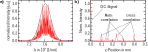
\includegraphics{figures/20_Theory/Optical/OCTspectrum.pdf}
      \caption{	\textbf{a)} Spectral interferogram of a swept source laser with gaussian amplitude profile when used in OCT with no sample (blue) and with three discrete reflectors in the sample arm (red).
				\textbf{b)} A-scan calculated from the spectral interferogram in a) using the Fourier transform.
				Modified with permision from \cite{Kretschmer}}
      \label{fig:OCTspectrum}
\end{figure}

The ability of an SS-OCT system to resolve two reflective surfaces separated by a small \textit{z} distance, termed \textit{axial resolution} $\delta z$, improves with a wider wavenumber sweep range $\Delta k$, following

\begin{equation}
\delta z = \frac{2 \sqrt{\rm{ln} (2)}}{\Delta k}.
\end{equation}

The ability of the system to resolve two adjacent points, i.e. its \textit{lateral resolution}, is independent of the axial resolution and completely determined by the optical system, as described in the next paragraphs. 

\subsection{Optical imaging and information transfer}
OCT imaging uses a conventional optical system to illuminate and collect the backscattered photons from the sample. As such, it is affected by diffraction effects, which perform a spatial low-pass filtering of the object, limiting the imaging resolution.

\subsubsection{Imaging in spatial domain: The PSF}

To understand this phenomenon it is useful to resort to the concept of Point Spread Function (PSF). The PSF is the 3 dimensional image that a optical system creates from an infinitesimal object. Therefore, it can be considered as the impulse response of the system. As any object $f(x,y,z)$ can be described as a set of infinitesimally small points, its image can be computed as the convolution -- or blurring -- of each point of the object with the PSF of the optical system \cite{Boreman2001}:
\begin{equation}
b(x,y,z) = f(x,y,z)\ast PSF(x,y,z)
\label{eq:imaging}
\end{equation}

\subsubsection{Imaging in frequency domain: The MTF}

It is also possible to describe this blurring in spatial frequency domain. Here, the imaging process is modeled as a low-pass filtering of the frequency content of the object. If the object is described by its frequency content or spectrum $F(\bm{k})$ and the modulation transfer function $MTF(\bm{k})$ describes the optical filtering, the frequency content of the incoherent image can be calculated as
\begin{equation}
B(k_x,k_y,k_z) = F(k_x,k_y,k_z) \cdot MTF(k_{x},k_{y},k_{z}).
\end{equation}

Notice that in the frequency domain, the spectrum of the object has to be simply multiplied by the MTF of the system, instead of convolved. Thus, working in the frequency domain eases the analysis of optical systems.


\subsection{Relation between PSF, ESF and MTF}
There is a fundamental mathematical relation between the MTF and the PSF: the MTF is the real part of the fourier transform of the PSF, i.e. the Optical Transfer Function (OTF) \cite{Boreman2001}:

\begin{equation}
OTF = \mathcal{F}(PSF)=\rm{MTF}\exp(- \mathit{i} \rm{PTF}).
\end{equation}

This relationship is exemplified in \autoref{fig:PSF_MTF}, where a PSF - MTF pair of a gaussian beam is shown.

\begin{figure}[h!]\centering 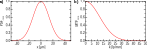
\includegraphics{figures/20_Theory/Optical/imaging/PSF_MTF.pdf}
      \caption{	\textbf{a)} Simulated PSF of a gaussian beam focused by a lens.
				\textbf{b)} Corresponding MTF obtained through a fourier transform. 
				}
      \label{fig:PSF_MTF}
\end{figure}

Measuring the PSF experimentally has the difficulty of requiring an "infinitesimally small" object to act as a \textit{delta} function. To ease the process, it is possible to use an object with a \textit{step} function, i.e. a sharp edge. The response of the system in this case is the convolution of the PSF with the \textit{step} function 
\begin{equation}
[\mathrm{Step}(x)1(y)]\ast \mathrm{PSF}(x,y) = \mathrm{ESF}(x))
\end{equation}
and its result denominated Edge Spread Function ESF \cite{Boreman2001}. 

As the convolution with a \textit{step} function is equivalent to integration, we find that 
\begin{equation}
\int \mathrm{PSF}(x) dx = \mathrm{ESF}(x).
\end{equation}

Thus, by simply differentiating the ESF it is possible to obtain the PSF, and by fourier tranform, the MTF of the system experimentally.

\subsection{Confocal Laser scanning microscopy (CLSM)}

The imaging topology used in this work is denominated Confocal Laser Scanning Microscopy (CLSM). This technique, represented in \autoref{fig:thConfSetup}, uses a fiber coupled laser source to project a focused beam in the sample. Some of the backscattered light from the sample is collected back to the fiber and detected by a photodiode. By scanning the focus position through the sample it is possible to obtain 2D or 3D images.

\begin{figure}[h!]\centering \includegraphics{figures/20_Theory/Optical/confSetup.pdf}
      \caption{			}
      \label{fig:thConfSetup}
\end{figure}

\subsubsection{Modeling of CLSM}

To understand the optical modeling of a CLSM we begin considering the probe as an illumination device, i.e. a projector. In this case, laser light coming from the optical fiber will be focused by the optical system in a plane located at its working distance. The focused spot won't be infinitesimally small due to two reasons: first, as in any optical system, diffraction takes place and blurs it with its $PSF_{\rm{optics}} (\mathbf{r})$, defined by the NA and the wavelength of the focused beam. Furthermore, the gaussian intensity distribution at the core of the fiber has a certain extent, characterized by its Mode Field Diameter (MFD). Once projected in the image plane, the MFD will be magnified by the optical system by a factor of $1/M$, where \textit{M} is the magnification of the beam defined as $f_\mathrm{fiber}/f_\mathrm{objective}$. This gaussian spot can be conceptually considered as the PSF due to the extended core of a fiber $PSF_{\rm{core}}$.

Thus, the projected spot, whose distribution is determined by the extended source of the fiber and the magnification and diffraction of the optical system, can be considered as the illumination PSF, calculated by convolution as
\begin{equation}
PSF_{\rm{ill}}(\bm{r}) = PSF_{\rm{core}}(\bm{r}M) \ast PSF_{\rm{optics}} (\bm{r})
\end{equation}
or equivalently, the illumination MTF
\begin{equation}
MTF_{\rm{ill}}(\mathbf{k}) = MTF_{\rm{core}}(\bm{k}/M) \cdot MTF_{\rm{optics}} (\bm{k} )
\end{equation}
following the PSF-MTF relationship. This behavior can be observed in \autoref{fig:MTFcomplete}a, where $MTF_{\rm{core}}$ and $MTF_{\rm{optics}}$ are simulated according to the design values of this work.

\begin{figure}[h!]\centering 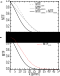
\includegraphics{figures/20_Theory/Optical/imaging/MTFcomplete.pdf}
      \caption{	\textbf{a)} Simulated MTF of the illumination or collection of a single point using the proposed optical system. The collection MTF is limited by the finite size of the fiber core and the diffraction of the optical system.
				\textbf{b)} MTF of the imaging system, calculated as the convolution of illumination and detection MTFs. 
				}
      \label{fig:MTFcomplete}
\end{figure}

The next step in the description of the CLSM considers the detection or collection of the backscattered light. If all the light coming from the fiber is projected in the $PSF_{\rm{ill}}$, we can use the Helmholtz reciprocity property of light to state that the photons originating within this PSF will be collected by the fiber and detected by the photodiode. Thus, the detection PSF is equivalent to the illumination PSF,
\begin{equation}
PSF_{\rm{det}}(\bm{r}) = PSF_{\rm{ill}}(\bm{r}) = PSF_{\rm{core}}(\bm{r}M) \ast PSF_{\rm{optics}} (\bm{r})
\end{equation}
or equivalently,
\begin{equation}
MTF_{\rm{det}}(\mathbf{k}) = MTF_{\rm{ill}}(\mathbf{k}) = MTF_{\rm{core}}(\bm{k}/M) \cdot MTF_{\rm{optics}} (\bm{k} )
\end{equation}

Considering now the complete imaging process of a confocal laser scanning microscope, a photon traveling through the fiber is projected inside the $PSF_{\rm{ill}}$, with a higher probability of illuminating the focus position. After being scattered by the sample, it has a high probability of being collected by the detector, as it is also in the center of the $PSF_{\rm{det}}$. It can be concluded that both PSFs are multiplied together, and thus the complete imaging system \textit{PSF} given by 
\begin{equation}
PSF_{\rm{sys}}(\bm{r}) = PSF_{\rm{ill}}(\bm{r}) \cdot PSF_{\rm{det}}(\bm{r}) \simeq PSF_{\rm{det}}(\bm{r})^2
\end{equation}
or equivalently, using the autoconvolution - squaring equivalence between spatial and frequency domain
\begin{equation}
MTF_{\rm{sys}}(\mathbf{k}) = MTF_{\rm{ill}}(\mathbf{k}) \ast MTF_{\rm{det}}(\mathbf{k}) \simeq AC[MTF_{\rm{det}}(\mathbf{k})].
\end{equation}
These operations are numerically calculated in \autoref{fig:MTFcomplete}b.

Finally, the resultant image can be calculated following \autoref{eq:imaging}:
\begin{equation}
b(\bm{r}) = f(x',y',z')\ast PSF_{\rm{sys}}(x',y',z').
\end{equation}

\subsubsection{Resolution of CLSM}

A final word regarding the resolution of CLSM: the autoconvolution of the PSF which characterizes CLSM can lead to an increase in resolution compared with conventional microscopy \textit{if the system is diffraction limited}. That implies using an illumination source and an detection aperture with pinholes siginificantly smaller than the diffraction limited PSF in these surfaces, so that $PSF_{\rm{core}}$ becomes a delta function and $PSF_{\rm{ill}}(\bm{r}) = PSF_{\rm{optics}} (\bm{r})$. 

In this work, the pinhole is defined by the diameter of the GRIN lens, which truncates the collimated beam at its $1/e^2$ level, corresponding with a truncation factor $k=1$. This limits the resolution of the system compared with a fully confocal system, as seen in \ref{fig:fullPartialConfocal}.

\begin{figure}[h!]\centering \includegraphics{figures/20_Theory/Optical/imaging/fullPartialConfocal.pdf}
      \caption{	Comparison of the simulated MTF of a confocal system with infinitesimally small pinhole (black) and with a pinhole with a truncation factor \textit{k} equal to 1 ($D = D_{\rm{beam,}1/e^2}$), red. The shaded area represents the possible MTFs for any truncation factor.}
      \label{fig:fullPartialConfocal}
\end{figure}

\section{Mechanics of fiber scanners}

The previous section focused in the acquisition of the depth information of a single column of a sample. But, in order to acquire a full, 3D volume of the sample, a 2D scanning mechanism is required. This section briefly goes over the physics and fundamental aspects of piezoelectric tube fiber scanners, starting with their actuation mechanism followed by the analytical modeling of their resonant scanning fiber.

\subsection{Piezoelectric tube actuators}
A piezoelectric tube is a solid state actuator consisting of a tube made of radially polarized piezoelectric material with inner and outer electrodes, as depicted in \autoref{fig:pztTheory}a. 
\begin{figure}[h!]
      \centering
      \includegraphics{figures/20_Theory/Mechanical/pztTheory.pdf}
      \caption{	\textbf{a)} Render of a piezoelectric tube.
      			\textbf{b)} Half-cut drawing of a piezoelectric tube in actuated state. The radial polarization of the piezoelectric material is shown in gray arrows. A voltage $\pm u_\mathrm{y}(t)$ is applied to the top and bottom outer electrodes, creating a radial electric field under those electrodes, depicted as red arrows. Due to the piezoelectric effect, the top of the tube contracts, while the bottom expands, inducing a bending of the tube.
      			\textbf{c)} Electrical model of the piezoelectric tube with four electrodes.}
      \label{fig:pztTheory}
\end{figure}
The outer metallization of the tube is divided in four quarter electrodes, which generate a radial electric field in the sandwiched portion of the piezoelectric material, shown in \autoref{fig:pztTheory}b. If a voltage difference is applied to two opposite electrodes of the tube, one side will contract while the other will expand due to the piezoelectric effect. This behavior is modeled \cite{Arnau2008} linearly by $\epsilon = d_{31} E$, where $\epsilon$ represents the in-plane strain, $d_{31}$ the piezoelectric strain coefficient, and \textit{E} the out-of-plane electric field magnitude. This asymmetry creates a bending moment across the axis of the tube, inducing its deformation. If one end of the actuator is kept static, the tip of the actuator will deflect and tilt according to the applied voltage. A 2D scanner can be created out of this setup if two independent signal control the horizontal and vertical electrodes, as shown in \autoref{fig:pztTheory}c.

The deflection of the tip of the tube is linear with the applied voltage, and in case of bipolar operation, estimated by \cite{Chen} to be
$$ \Delta y = V  \frac{2 \sqrt{2} d_{31} L^2}{\pi D h} $$
, where \textit{V} is the applied voltage to each opposing electrode, $d_{31}$ is the piezoelectric strain coefficient of the material in direction perpendicular to the polarization direction, \textit{L} is the length of the tube, \textit{D} its outer diameter and \textit{h} the thickness of its wall. Thus, longer tubes with a thinner diameter and wall thickness maximize the deflection of the tip. Typical deflections for small actuators lie in the order of $\SI{20}{\nano\meter / \volt}$.


\subsection{Resonant Beam Theory}
\label{sec:EB}
The piezoelectric actuator described in the last paragraphs couples mechanical energy into the cantilever of the scanner, formed by a fiber optic segment to which a GRIN lens is glued, as depicted in \autoref{fig:EB}a. As the scanner uses mechanical resonance to amplify the small displacements of the actuator, it is important to model the resonance frequency of such a system. 

\begin{figure}[h!]\centering
      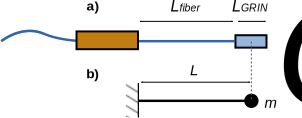
\includegraphics{figures/20_Theory/Mechanical/EB.pdf}
      \caption{\textbf{a)} Drawing of the piezoelectric scanner: piezoelectric tube, fiber and GRIN lens. 
      \textbf{b)} Simplified mechanical diagram obtained by modeling the fiber as a weightless cantilever and the GRIN lens as a point mass.}
      \label{fig:EB}
\end{figure}

The fiber-GRIN assembly can be modeled as a point-loaded, fixed-free cantilever and the GRIN lens weight can be concentrated in its center of gravity, as represented in Figure \ref{fig:EB})b. 

Now, by applying the ideal mass-spring harmonic resonator equation, the resonance frequency can be estimated as 
\begin{equation}
f_\mathrm{res} = \frac{1}{2 \pi} \sqrt{\frac{K_\mathrm{cantilever}}{m_{\mathrm{GRIN}}}} 
\label{eq:fres}
\end{equation}
where $K_\mathrm{cantilever}$ represents the elastic constant of the fiber cantilever. Considering it as a fixed-free, point loaded cantilever, its spring constant can be calculated as 
\begin{equation}
K_\mathrm{cantilever} = \frac{3 E I}{L^3} = \frac{3 \pi}{4} \frac{E_\mathrm{fiber} r_\mathrm{fiber}^4}{L^3}
\label{eq:EB}
\end{equation}
following the Euler-Bernoulli theory \cite{MarcJ.Madou2011} and considering that the moment of inertia of the cylindrical fiber is given by $I_\mathrm{fiber} = \frac{\pi}{4} r^4$. 
